\chapter{自动机}

\vspace{-5pt}
\begin{center}
    \pgfornament[width=0.36\linewidth,color=lsp]{88}
\end{center}
\section{图结构的引入}
\begin{definition}[一阶逻辑公式]
\begin{itemize}
    \item 逻辑操作符:合取($\wedge $),析取($\vee$),否定($\neg$),蕴含($\rightarrow$)
    \item 量词操作符:全称量词($\exists$),存在量词($\forall$)
\end{itemize}
\end{definition}
\begin{definition}[Kripke structure]
令AP为原子命题,则AP上的四元组$\mathcal{M}$称之为Kripke结构,$\mathcal{M}=\left(S,S_0,R,L\right)$,其中
\begin{enumerate}
    \item $S$是有限的集合,内部的每个元素均为一个状态,即状态的有限集,
    \item $S_0 \subseteq S$ 是初始的状态集合,
    \item $R \subseteq S \times S$ 是变迁关系,
    \item $L: S \rightarrow 2^{AP}$为标识函数,标识在某个状态下为真的原子命题集。
\end{enumerate}
\end{definition}

\begin{definition}[transition system]
转移系统(transition system)通常用于描述系统的行为,是一种有向图,节点代表状态,边代表状态的变化。
转移系统$TS$是一个六元组$ TS = \left(S,Act,\rightarrow,S_0,AP,L\right)$。
\begin{itemize}
    \item $S$是状态的集合,
    \item $Act$是一组动作的集合,
    \item $\rightarrow \subseteq S \times Act \times S$ 是变迁关系,
    \item $S_0 \subseteq S$ 是初始的状态集合,
    \item $AP$是一组原子命题的集合,
    \item $L: S \rightarrow 2^{AP}$为标识函数,标识在某个状态下为真的原子命题集。
\end{itemize}
相关概念:
\begin{enumerate}
    \item 直接后继(direct successors):指当前状态通过执行动作$\alpha$ 的所能达到的状态集合。
    $$
    {Post}(\mathrm{s}, \alpha)=\left\{\mathrm{s}^{\prime} \in \mathrm{S} \mid \mathrm{s} \stackrel{\alpha}{\longrightarrow} \mathrm{s}^{\prime}\right\}
    $$
    若对$\alpha$不进行限制,则
    $$
    {Post}(\mathrm{s})=\bigcup_{\alpha \in \text { Act }} \operatorname{Post}(\mathrm{s}, \alpha)
    $$
    \item 直接前任(direct predecessors):指通过执行动作$\alpha$ 到达当前状态的状态集合。
    $$
    {Pre}(\mathrm{s}, \alpha)=\left\{\mathrm{s}^{\prime} \in \mathrm{S} \mid \mathrm{s}^{\prime} \stackrel{\alpha}{\longrightarrow} \mathrm{s}\right\}
    $$
    若对$\alpha$不进行限制,则
    $$
    {Pre}(\mathrm{s})=\bigcup_{\alpha \in \text { Act }} \operatorname{Pre}(\mathrm{s}, \alpha)
    $$
    \item 确定性
    \begin{itemize}
    \item 动作确定性:动作转移唯一,即出度唯一
    $$
    \left|\mathrm{S}_0\right| \leq 1 \text { and }\left|\mathrm{Post}(\mathrm{s}, \alpha)\right|| \leq 1
    $$
    \item AP确定性:动作转移到的AP确定
    $$
    \left|\mathrm{S}_0\right| \leq 1 \text { and }\left|\mathrm{Post}(\mathrm{s}, \alpha) \cap\left\{\mathrm{s}^{\prime} \in \mathrm{S} \mid \mathrm{L}\left(\mathrm{s}^{\prime}\right)=\mathrm{A}\right\}\right| \leq 1\left(\mathrm{~A} \in 2^{\mathrm{AP}}\right)
    $$
    \end{itemize}
\end{enumerate}
\end{definition}

\begin{definition}[Program Graph]
Program Graph 由六元组 $\mathcal{PG}=\left(Loc,Act,Effect,\hookrightarrow,Loc_{0},g_{0}\right)$,其中
\begin{enumerate}
    \item $Loc$是位置的集合,
    \item $Act$是动作的集合,
    \item $Effect \text{:}Act \times Eval(Var) \rightarrow Eval(Var)$ 是变迁关系,
    \item $\hookrightarrow \subseteq Loc \times Cond(Var) \times Act \times Loc$ 是条件转移关系的集合,
    \item $Loc_{0} \subseteq Loc$为初始的位置集合,
    \item $g_{0} \subseteq Cond(Var)$ 是初始的条件。
\end{enumerate}
相比于Transition system,Program Graph 移除了状态的概念,引入了条件与位置,即转移时跟位置、当前的条件以及动作均有关系。
\end{definition}

\section{状态机与正则语言}
\begin{definition}[前置知识]
\begin{enumerate}
    \item 符号,如:$a,b,c, 0, 1, 2$。
    \item 字母表(alphabet),字母表$\Sigma$是符号的集合,如${a,b}, {0,1,2}$。
    \item 字符串(string)为符号的序列,如$a,ab,aba$。
    \item 语言(language)为字符串的集合,如${00,11,01,10}$。
    \item 字母表的幂(power),$\Sigma_{n}$表示长度为$n$的字符串的集合。$\Sigma^{n}=\Sigma_{0}
    \cup \Sigma_{1} \cup \Sigma_{2}\dots$
\end{enumerate}
\end{definition}

\subsection{有限状态机}
有限状态机(finite state machine)又被称为有限自动机(finite automata),可以根据有无输出分为以下两类:
\begin{itemize}
    \item 有输出的有限状态机:Moore Machine,Mealy Machine
    \item 无输出的有限状态机:DFA,NFA,$\epsilon$-NFA
\end{itemize}

其中,Moore Machine 的输出位于状态,Mealy Machine 的输出位于转换。
可以根据确定性为以下两类:
\begin{itemize}
    \item 确定性有限状态机:DFA
    \item 非确定性有限状态机:NFA,$\epsilon$-NFA
\end{itemize}

其中,NFA可以转化为DFA。

\section{系统属性与规约}
\subsection{线性时间属性}
线性时间属性指定了过渡系统应该显示的轨迹。非正式的说明,线性时间属性制定了所考虑系统的可允许(或者说期望)的行为。

路径:转移系统(TS)上的路径片段被定义为有限或无限的状态序列;最大路径片段为结束于终止状态的有限路径片段或无限路径片段。

执行:转移系统(TS)上的执行被定义为状态和动作的序列,即
$\mathrm{s}_0 \stackrel{\alpha_0}{\longrightarrow} \mathrm{s}_1 \stackrel{\alpha_1}{\longrightarrow} \ldots$。

迹(traces):当前状态为真的原子命题组成的序列,即$L(S_0)L(S_1)L(S_2)\dots$。

线性时间属性是TS中迹的要求,所以AP上的线性时间属性是$(2_{AP})_w$的子集。

若转移系统满足线性时间属性$\mathrm{P}$,那么表明 $ TS \models P \text{当且仅当} Traces(TS) \subseteq  P $。
线性时间属性$P$刻画了$AP$上能够出现的原子命题序列,而迹表示系统在$AP$上出现的原子命题序列,若系统的迹是$P$的子集,
那么系统满足了线性时间属性。
\subsection{安全性和不变性}
安全性通常被描述为“不会发生不好的事情”(nothing bad should happen)。
不变性是安全性的子集,若在$AP$上的线性属性$P_{inv}$具有不变性,那么具备如下形式:
\begin{equation}
    P_{inv} = \{A_{0}A_{1}A_{2}\ldots \in(2^{AP})^{w}\vert \forall j>=0, A_{j} \models \Phi \}
\end{equation}
不变性是线性时态属性,系统所有可达的状态均满足属性$\Phi$。

安全性除了对可达的状态有一定的要求,还对一定长度的路径片段有要求,可被定义为如下形式:
\begin{equation}
   \forall \sigma \in (2^{AP})^(w) \setminus  P_{safe} \text{,} \exists \sigma \text{的有限前缀}\hat{\sigma}\text{满足}
    P_{safe} \cap \{ \sigma^{\prime} \in (2^{AP})^w| \hat{\sigma}  \text{是} \sigma^{\prime} 的有限前缀\} = \varnothing \emptyset 
\end{equation}
对于所有的无限字$\sigma = A_{0}A_{1}A_{2}\ldots \in (2^{AP})^{w} \setminus P_{safe}$,存在有限前缀$\hat{\sigma} = A_{0}A_{1} \dots A_{n}$,
使得以$\hat{\sigma}$ 为前缀起始的字不属于$P_{safe}$。
其中有限字$\hat{\sigma} = A_{0}A_{1} \dots A_{n}$被称为$P_{safe}$的坏前缀,符号表示为$BadPref(P_{safe})$。
\subsection{安全性和活性}
\begin{definition}[Closure]
线性时间属性$P$的闭包定义为:
$$
closure(P) = \{ \sigma \in (2^{AP})^{w} \vert  pref(\sigma) \subseteq pref(P)\}
$$
\end{definition}
若$P$是安全属性,当且仅当$closure(P) = P$。
若$P_{live}$是$AP$上的活性,那么在任意时刻:
$$
Pref(P_{live}) = (2^{AP})^{*}
$$
$P_{live}$被称为活性,那么每个在AP的有限字都能扩展称为$P_{live}$中的无线字。
线性时间属性的分类:
\begin{figure}
\centering %图片居中
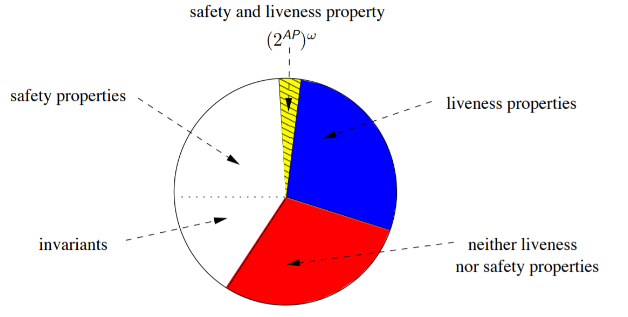
\includegraphics[scale = 0.5]{./automaton/figures/LTProperty.png} %插入图片,[]中设置图片大小,{}中是图片文件名
\caption{线性时间属性分类} %最终文档中希望显示的图片标题   
\end{figure}
不变性包含于安全性,安全性与活性存在相交部分,也有部分属性既不属于安全性也不属于活性。

\section{马尔可夫决策过程}
\begin{definition}[MDP]
带标签的马尔可夫决策过程是一个元组$\mathcal{M} =(S,A,P,s_0,AP,L) $,
\begin{itemize}
\item $S$是有限状态的集合;
\item $A$是有限动作的集合;
\item $P:S\times A\times S \rightarrow [0,1]$是概率转移函数;
\item $s_0 \in S$是初始状态;
\item $L:S \rightarrow 2^{AP}$是一个标签函数。
\end{itemize}
一条路径指的是一条无限长的状态序列 $ \sigma  = s_0 s_1 s_2 \dots$,其中
$s_i \in S$使得对于任意$i \geqslant 0 $,存在$a_i \in A$且$P(s_i,a_i,s_{i+1}) > 0 $。
我们使用$\sigma[i]$表示状态$s_i$,同时使用$\sigma[:i]$和$\sigma[i+1:]$分别表示
前缀$s_{0}s_{1} \dots s_{i}$和后缀$s_{i+1}s_{i+2}\dots$。
\end{definition}
\begin{definition}[Policy]
马尔可夫决策过程上的策略$\pi$是映射函数$\pi:S^{+}->A$使得对于任意的路径$\sigma$存在$\pi(\sigma[:n])=\pi(\sigma[n])$。
若策略为无记忆性的(memoryless),则该策略只依赖于当前的状态,即$\pi:S->A$。
一个由无记忆性的策略诱导的马尔可夫链为一个元组$\mathcal{M}_{\pi}=(S,P_{\pi},s_0,AP,L) $,其中$P_{\pi}(s,s^{\prime})=P(s,\pi(s),s^{\prime})$。
马尔可夫链的底部强连通分量(bottom strongly connected component,BSCC)是一个无向外转移的强连通分量。
\end{definition}

\section{线性时态逻辑}
线性时态逻辑(LTL)提供了高级语言来描述系统规约。LTL可被归纳的构造为布尔(boolean)运算,
取反运算,析取运算等逻辑运算以及Next($ \bigcirc $),Until($U$)等时态运算。
LTL的语法如下:
\begin{equation}
    \varphi::=\operatorname{true}|a| \varphi_1 \wedge \varphi_2|\neg \varphi| \bigcirc \varphi \mid \varphi_1 U \varphi_2, a \in \mathrm{AP}
\end{equation}
\begin{definition}
若关于MDP的一条路径$\sigma$满足LTL的规约$\varphi$,可表示为$\sigma \models \varphi$。关于路径$\sigma$上的
状态$s_0 s_1 \dots s_n$产生的$AP$序列$L(s_0) L(s_1) \dots L(s_n)$存在满足LTL的规约。
\end{definition}

\section{自动机}

\begin{definition}[Limit-Deterministic Büchi Automata(LDBA)]
极限确定性Büchi自动机是一个元组$\mathcal{A} =(Q,\Sigma ,\delta ,q_0,B) $,
\begin{itemize}
    \item $Q$是有限状态的集合;
    \item $\Sigma$是有限字母表;
    \item $\delta:Q\times (\Sigma \cup \{\epsilon\})\times S \rightarrow [0,1]$是部分转移函数;
    \item $q_0 \in S$是初始状态;
    \item $B$是一个接受状态的集合。
\end{itemize}
其中,$\sigma$ 是不包含$\epsilon - moves$全移动,也就是说对于
所有的$q\in Q$,$\alpha \in \Sigma$,$|\sigma(q,\alpha)| = 1$;除此之外$Q$必须可分为初始组件和接受组件,
即$Q_I \cup Q_A=Q$,并且$\epsilon - moves$不允许在接受组件中,也就是对于任意$q \in Q_A$,
$\sigma(q,\epsilon) = \emptyset$,接受组件内的状态只允许内部转移,所有的接收状态$B$包含在$Q_A$内。
一条无限长的路径被LDBA接受如果满足Büchi condition,也就是$inf(\sigma) \cap B \neq \emptyset $,其中
$inf(\sigma)$ 表示该状态集合被$\sigma$访问无限次。
\end{definition}

\subsection{搭建马尔可夫决策与自动机的桥梁}
\begin{definition}[Product MDP]
乘积马尔可夫决策过程 $\mathcal{M}^{\times}=\left(S^{\times}, A^{\times}, P^{\times}, s_0^{\times}\right.$, $\left.B^{\times}\right)$
是由一个 $M D P$ $\mathcal{M}=\left(S, A, P, s_0, A P, L\right)$ 和一个 $L D B A$ $\mathcal{A}=\left(Q, 2^{A P}, \delta, q_0, B\right)$ 组成,
可被定义为:
\begin{itemize}
    \item $S^{\times}=S \times Q$ 是状态集合,
    \item $A^{\times}=A \cup A^\epsilon, A^\epsilon:=\left\{\epsilon_q \mid q \in Q\right\}$是动作集合,
    \item $P^{\times}: S^{\times} \times A^{\times} \times S^{\times} \rightarrow[0,1]$是转移函数,
    $$
    P^{\times}\left(\langle s, q\rangle, a,\left\langle s^{\prime}, q^{\prime}\right\rangle\right)
    = 
    \begin{cases}
    P\left(s, a, s^{\prime}\right) & q^{\prime}=\delta(q, L(s)) \text { and } a \notin A^\epsilon 
    \\ 1 & a=\epsilon_{q^{\prime}} \text { and } q^{\prime} \in \delta(q, \epsilon) \text { and } s=s^{\prime}, 
    \\ 0 & \text { otherwise }
    \end{cases}
    $$
    \item $s_0^{\times}$是由$\left\langle s_0, q_0\right\rangle$组成,
    \item $B^{\times}=\left\{\langle s, q\rangle \in S^{\times} \mid q \in B\right\}$是接受状态的集合
\end{itemize}
乘积自动机$\mathcal{M}^{\times}$上的路径$\sigma$ 满足 Büchi condition,即 $inf(\sigma) \cap B^{\times} \neq \emptyset$.
\end{definition}

\begin{problem}[Max Satisfaction]
给定MDP $\mathcal{M} =(S,A,P,s_0,AP,L)$,其中$P$信息未知。设计一个无模型
\end{problem}